\chapter{Methodik}\label{chap:methodik}

In diesem Kapitel werden in \hyperref[sec:daten]{Abschnitt 5.1} zunächst die zum Training und zur Evaluation verwendeten Datensätze und in \hyperref[sec:vorverarbeitung]{Abschnitt 5.2} deren Vorverarbeitung beschrieben. Anschließend wird in \hyperref[sec:architektur]{Abschnitt 5.3} der in dieser Arbeit verwendete Ansatz für ein \gls{DL}-Modell beschrieben. Zuletzt wird in \hyperref[sec:trainingsprozess]{Abschnitt 5.4} auf die Umsetzung dieses Modells genauer eingegangen.

\section{Genutztes Datenmaterial}\label{sec:daten}

In dieser Arbeit wurden vier Datenbanken genutzt: die xECGArch-Datenbank \cite{goettling_xecgarch_2024}, Icentia11k \cite{tan_icentia11k_2021} \cite{tan_icentia11k_2022}, \gls{SHDB-AF} \cite{tsutsui_shdb-af_2024} \cite{tsutsui_shdb-af_2024-1} und eine Datenbank, welche aus dem TIMELY-Datensatz \cite{schmitz_patient-centered_2022} erstellt wurde.

\subsection*{xECGArch-Datenbank}
Für das Training der Modelle wurde die von Goettling et al. \cite{goettling_xecgarch_2024} für  xECGArch erstellte Datenbank verwendet.  
Die xECGArch-Datenbank wurde zusammengesetzt aus den Datenbanken PTB-XL \cite{wagner_ptb-xl_2020} \cite{wagner_ptb-xl_nodate}, Chapman-Shaoxing \cite{zheng_12-lead_2020} \cite{zheng_large_nodate}, Georgia-12-Lead \cite{perez_alday_classification_2020} \cite{perez_alday_classification_nodate} und \gls{CPSC2018} \cite{liu_open_2018}. 
Sie enthält $4~927$ als \gls{VHF} annotierte, sowie $4~927$ als nicht-\gls{VHF} annotierte Aufnahmen. $429$ der nicht-\gls{VHF}-Aufnahmen enthalten einen normalen Sinusrhythmus, Sinus Tachykardie oder Sinus Bradykardie. Die genaue Zusammensetzung der Datenbank aus den Ursprungsdatenbanken kann in \hyperref[tab:Klassenverteilung_xECG]{Tab.~5.1} nachgelesen werden.
Die xECGArch-Datenbank ist aufgeteilt in ein Trainingsset mit $4~420$ \gls{VHF}- und $4~448$ nicht-\gls{VHF}-Aufnahmen, welches für das Training der Modelle in dieser Arbeit genutzt wurde, sowie ein Testset mit $507$ \gls{VHF}- und $479$ nicht-\gls{VHF}-Aufnahmen, welches für die Evaluation in \hyperref[chap:Ergebnisse]{Kapitel 6} genutzt wurde. Die Aufnahmen haben eine Abtastrate von 500~Hz. \cite{goettling_xecgarch_2024}

\begin{table}[h!]
\centering
\caption[Klassenverteilung der xECGArch-Datenbank]{Anzahl und Ursprungsdatenbank der \gls{EKG}-Aufnahmen in der xECGArch-Datenbank. AF steht für Vorhofflimmern, NSR für normalen Sinusrhythmus, ST für Sinustachykardie ohne andere Annotation, SB für Sinusbradykardie ohne andere Annotation und Other umfasst alle anderen Rythmusstörungen. Entnommen aus \cite{goettling_xecgarch_2024}. }
\label{tab:Klassenverteilung_xECG}
\begin{tabular}{lccccc}
\toprule
\textbf{Klasse}       & \multicolumn{5}{c}{\textbf{Datenbank}} \\ 
\cmidrule(lr){2-6}
                     & \textbf{PTB-XL} & \textbf{Georgia} & \textbf{CPSC2018} & \textbf{Chapman-} & \textbf{Total} \\
                     &                 &                  &                   & \textbf{Shaoxing} &                \\ 
\midrule
\textbf{NSR, ST, SB} & 290             & 67               & 12                & 123               & 492            \\
\textbf{OTHER}       & 169             & 2~032            & 1~921             & 313               & 4~435          \\
\textbf{AF}          & 1~497           & 553              & 1~097             & 1~780             & 4~927          \\
\bottomrule
\end{tabular}
\end{table}

%TODO warum balanciert
%TODO 12 Kanal EKGs

\subsection*{Icentia11k}
Da das Ziel dieser Arbeit die Entwicklung eines \gls{DL}-Modells ist, welches robust gegen signalmorphologische Veränderungen bei Aufnahmen mobiler \gls{EKG}-Patches ist, werden zur Evaluation Datenbanken mit Aufnahmen solcher Patches benötigt.
Die Icentia11k-Datenbank~\cite{tan_icentia11k_2021}~\cite{tan_icentia11k_2022} ist zusammengesetzt aus Aufnahmen von 11~000 unterschiedlichen Patienten, welche mit dem CardioSTAT\footnote{https://www.cardiostat.com/} \gls{EKG}-Patch \cite{paquet_adhesive_2022} aufgezeichnet wurden. Dabei handelt es sich um einen Ein-Kanal-Patch, welches mittig auf dem Brustkorb angebracht wird und eine maximale Tragedauer von zwei Wochen hat. Die Aufnahmen der Patienten wurden in ca. einstündige Segmente zerlegt und von Technologen der Icentia inc. (Qu\'ebec, Canada) annotiert. Mögliche Rhythmus-Label sind NSR für normalen Sinusrhythmus, AFib für \gls{VHF} und AFlutter für Vorhofflattern. Einige Abschnitte sind nicht annotiert. Insgesamt gibt es $542~157$ Segmente mit einer Abtastrate von 250~Hz. \cite{tan_icentia11k_2021}


\subsection*{SHDB-AF}

%TODO foto von elektrodenplazierungen bei den drei nicht standard ekg datenbanken

Die \gls{SHDB-AF}~\cite{tsutsui_shdb-af_2024}~\cite{tsutsui_shdb-af_2024-1} ist eine japanische Datenbank, die entwickelt wurde, um die Generalisierfähigkeit von \gls{DL}-Modellen über verschiedene Domain Shifts hinweg zu testen und eignet sich deshalb, um auch das in dieser Arbeit entwickelte Modell zu evaluieren. Die Datenbank setzt sich zusammen aus Aufnahmen von 100 unterschiedlichen Patienten, welche unter paroxysmalem \gls{VHF} leiden. Die Aufnahmen wurden mit dem Holter-Monitor der Fukuda Denshi~Co.,~Ltd.~(Tokyo, Japan) aufgezeichnet und enthalten zwei Kanäle, bei denen es sich um modifizierte CC5- und NASA-Ableitungen handelt. Die \gls{EKG}s sind ca. 24 Stunden lang und wurden mit einer Abtastrate von 125~Hz aufgezeichnet, vor der Veröffentlichung mit einem Bandpass mit den Grenzfrequenzen 0,67 und 100~Hz gefiltert und auf 200~Hz resampelt. Annotiert sind Abschnitte mit \gls{VHF} als AFIB, Vorhofflattern als AFL, Vorhoftachykardie als AT, Vorhofbradykardie als AB und andere supraventrikuläre Tachykardien als PAT oder NOD. Die übrigen Abschnitte erhielten das Label N. \cite{tsutsui_shdb-af_2024}



\subsection*{TIMELY-Datensatz}


%wie viele patienten

Die Daten des TIMELY-Datensatzes wurden im Rahmen des TIMELY Projektes erhoben. 
Ziel des Projekts ist die Entwicklung einer eHealth-Plattform, welche durch künstliche Intelligenz unterstützt wird 
und die Ärzten und Patienten als Hilfsmittel bei der Behandlung von Herzerkrankungen dient. 
Die \gls{EKG}s wurden mit dem net\_ECG-Patch der SEMDATEX GmbH (Berlin, Deutschland)\footnote{https://www.semdatex.com/de/externe-geraete}, welches drei \gls{EKG}-Ableitungen aufnimmt und über dem Herzen platziert wird, aufgezeichnet. Die Aufnahmen haben eine durchschnittliche Dauer von 24 Stunden und eine Abtastrate von 800~Hz. Die Daten sind nicht annotiert, sodass im Rahmen dieser Arbeit ein Datensatz erstellt und annotiert wurde. \cite{schmitz_patient-centered_2022} \cite{noauthor_patient-centered_nodate}


\section{Vorverarbeitung der Datensätze}\label{sec:vorverarbeitung}

Alle Datensätze wurden mit der Python Toolbox \texttt{Neurokit2} \cite{makowski_neurokit2_2021} vorverarbeitet. Gefiltert wurde mit einem Butterworth-Bandpass 4.Ordnung und den Grenzfrequenzen 0.5 und 150 Hz. Diese Grenzfrequenzen wurden ausgewählt, da die diagnostisch relevanten Informationen eines \gls{EKG}s sich innerhalb dieser Frequenzen befinden \cite{kligfield_recommendations_2007}. Genutzt wurde die Implementierung \texttt{butterworth\_ba} von Neurokit2, da diese weniger Randartefakte eingeführt hat als die alternative Implementierung \texttt{butterworth}. Anschließend wurde mit einem Powerline-Filter die Frequenz 50~Hz herausgefiltert. Zuletzt wurden die Daten z-normalisiert.
 
\subsection*{xECGArch-Datenbank}
%test_6lead.json
%train_6lead.json

Das Datenmaterial wurde von der PhysioNet-Website \cite{goldberger_physiobank_2000} zur \textit{PhysioNet/Computing in Cardiology Challenge 2020} \cite{perez_alday_classification_2020} \cite{perez_alday_classification_nodate} heruntergeladen. Genutzt wurden nur Aufnahmen mit mindestens 10 Sekunden Länge. Längere Aufnahmen wurden gekürzt, indem ein 10-Sekunden-Segment aus der Mitte der Aufnahme entnommen wurde. Von den 12 Kanälen der Aufnahmen wurden die Brustwandableitungen nicht verwendet, da sie morphologisch starke Unterschiede zu den Aufnahmen der \gls{EKG}-Patches aufweisen. Die Aufnahmen der meisten \gls{EKG}-Patches enthalten keine Brustwandableitungen, da sie auf Mobilität und einfache Platzierbarkeit ausgelegt sind. Das Einbeziehen der Brustwandableitungen in das Training des \gls{DL}-Modells kann daher kontraproduktiv sein, da das Modell lernen würde, sich auf Signaleigenschaften zu verlassen, die in den mobilen Aufnahmen nicht vorhanden sind. Die übrigen 6 Kanäle I, II, III, aVR, aVL und aVF wurden als einzelne Kanäle für das  Training genutzt.


\subsection*{Icentia11k}

Der Datensatz wurde von der PhysioNet-Website \cite{goldberger_physiobank_2000} heruntergeladen. Zu 363 Segmenten fehlte entweder die Header- oder Annotations-Datei, sodass diese Segmente nicht weiter betrachtet wurden. Um die Menge an Daten zu verringern und die Diversität des Datensatzes dennoch zu erhalten wurde von jedem Patienten ein zufälliges Segment ausgewählt. Aus diesem Segment wurde ein zufälliges 10-Sekunden-Fenster ausgewählt, wobei nicht-annotierte Abschnitte ignoriert wurden. Ist ein gesamtes Segment nicht annotiert, sodass kein 10-Sekun-den-Fenster extrahiert werden kann oder ist das einzige annotierte Intervall kürzer als 10 Sekunden, wird ein anderes Segment ausgewählt. Nach Auswahl der Fenster wurden diese auf 500~Hz mit linearer Interpolation resampelt und anschließend wie zuvor erwähnt gefiltert. Insgesamt gibt es 513 Fenster mit dem Label \gls{VHF} und 10~350 Fenster, die nicht mit \gls{VHF} gelabelt wurden. Die genaue Klassenzusammensetzung lässt sich in \hyperref[tab:Klassenverteilung_Icentia11k]{Tab.~5.2} nachlesen.

\begin{table}[h!]
\centering
\caption[Klassenverteilung im Icentia11k-Datensatz]{Anzahl und Label der 10-Sekunden-Fenster in dem für die Evaluation genutzten Ausschnitt aus der Icentia11k-Datenbank. NSR steht für normalen Sinusrhythmus, AFL für Vorhofflattern und AF für Vorhofflimmern.}
\label{tab:Klassenverteilung_Icentia11k}
\begin{tabular}{ll}
\hline
\textbf{Klasse} & \makecell{\textbf{Anzahl in Icentia11k}} \\ \hline
\textbf{NSR} & \makecell{10~176}   \\
\textbf{AFIB} & \makecell{513} \\
\textbf{AFL} & \makecell{174}  \\ \hline
\end{tabular}
\end{table}

\subsection*{SHDB-AF}

Die \gls{SHDB-AF} wurde von der PhysioNet-Website \cite{goldberger_physiobank_2000} heruntergeladen. Jede Aufnahme wurde auf 500~Hz mit linearer Interpolation resampelt, vollständig in 10-Sekunden-Fenster aufgeteilt und anschließend gefiltert. Insgesamt gibt es 167~288 Fenster mit dem Label \gls{VHF} und 688~090 Fenster, die nicht mit \gls{VHF} gelabelt wurden. Die genaue Klassenzusammensetzung lässt sich in \hyperref[tab:Klassenverteilung_SHDB]{Tab.~5.3} nachlesen. 

\begin{table}[h!]
\centering
\caption[Klassenverteilung in der SHDB-AF-Datenbank]{Anzahl und Label der zur Evaluation genutzten 10-Sekunden-Fenster in der \gls{SHDB-AF}-Datenbank. AFIB bedeutet \gls{VHF}, AFL Vorhofflattern, AT Vorhoftachykardie, AB Vorhofbradykardie und andere supraventrikuläre Tachykardien besitzen die Label PAT oder NOD. Alle übrigen Fenster wurden mit N gelabelt.}
\label{tab:Klassenverteilung_SHDB}
\begin{tabular}{ll}
\hline
\textbf{Klasse} & \makecell{\textbf{Anzahl in SHDB-AF}} \\ \hline
\textbf{N} & \makecell{672~084}   \\
\textbf{NOD} & \makecell{89}   \\
\textbf{PAT} & \makecell{117}   \\
\textbf{AT} & \makecell{2562}   \\
\textbf{AB} & \makecell{366}   \\
\textbf{AFL} & \makecell{12~872} \\
\textbf{AFIB} & \makecell{167~288}  \\ \hline
\end{tabular}
\end{table}

\subsection*{TIMELY-Datensatz} 

Die Rohdaten des TIMELY-Datensatzes wurden am Institut für Biomedizinische Technik der TU Dresden zur Verfügung gestellt. Die Verarbeitung, welche durchgeführt wurde, um aus den Rohdaten einen annotierten Datensatz zu erstellen, wird im Folgenden erklärt.
Es war den Patienten möglich, das EKG-Patch bspw. zum Duschen abzunehmen. Für die Zeitspanne, in der der Patch nicht angebracht war, wurde ein Rechtecksignal und anschließend eine Nullinie aufgezeichnet. Mit Hilfe einer Discard-Mask wurden diese Rechtecksignale, Nullinien, sowie zu niederamplitudige Signale entfernt. Die übrigen Segmente wurden mit Hilfe eines Ensembles aus einem Decision Tree Ensemble von Hammer et al. \cite{hammer_automatic_2021}, xECGArch \cite{goettling_xecgarch_2024} und einem von Ribeiro et al. entwickelten Modell \cite{ribeiro_automatic_2020} klassifiziert. Dafür wurden die Segmente entsprechend den drei Ansätzen vorverarbeitet und in 30- bzw. 10-Sekunden-Fenster zerlegt. Für die 10-Sekunden-Fenster wurden die Aufnahmen von 800~Hz auf 500~Hz mit Nutzung des Mittelwerts als Aggregationsverfahren resamplet. 

Die Patienten sind nicht gleichmäßig im Datensatz vertreten, da alle als \gls{VHF} klassifizierten Fenster aus Aufnahmen von 5 Patienten bestehen. Insgesamt gab es 2~007 als \gls{VHF} klassifizierte Fenster. Um den Datensatz zu erhalten wurden zufällig 2~100 als nicht-\gls{VHF} klassifizierte Fenster ausgewählt. 

Anschließend wurden die automatische Annotation manuell durch zwei Personen unabhängig überprüft. Ein Fenster wurde als \gls{VHF} annotiert, wenn zwei der drei zur Annotation berücksichtigten Parameter \textit{fehlende P-Welle}, \textit{F-Wellen} und \textit{absolute Arrhythmie} mit \textit{ja} beantwortet wurden. Wurden mindestens zwei der Parameter mit \textit{nein} beantwortet, wurde das Fenster mit nicht-\gls{VHF} annotiert. Im Falle von Uneinigkeit der Annotationen wurde das Fenster entfernt. Fenster, bei denen die Ableitung durch extrem starkes Rauschen unbrauchbar war, wurden entfernt. Dadurch entsteht eine leicht unterschiedliche Anzahl an verfügbaren Fenstern pro Ableitung. Die genaue Anzahl lässt sich in \hyperref[tab:Klassenverteilung_Timely]{Tab.~5.3} nachlesen.
Für diese Arbeit wurde der so erhaltene Datensatz aus 10-Sekunden-Fenstern wie zuvor beschrieben mit Neurokit2 gefiltert. 

\begin{table}[h!]
\centering
\caption[Klassenverteilung im TIMELY-Datensatz]{Anzahl und Label der 10-Sekunden-Fenster in dem für die Evaluation genutzten Timely-Datensatz. AF steht für Vorhofflimmern, OTHER für nicht-Vorhofflimmern.}
\label{tab:Klassenverteilung_Timely}
\begin{tabular}{lccc}
\toprule
\textbf{Klasse}       & \multicolumn{3}{c}{\textbf{Anzahl im Timely-Datensatz}} \\ 
\cmidrule(lr){2-4}
                     & \textbf{Ableitung 1} & \textbf{Ableitung 2} & \textbf{Ableitung 3} \\ 
\midrule
\textbf{OTHER}       & 2~303  & 2~284  & 2~245  \\
\textbf{AF}          & 1~660  & 1~660  & 1~661  \\
\bottomrule
\end{tabular}
\end{table}



 
%TODO in den daten vorhandene Distribution Shifts (welches kaptiel? -> grundladen)
% aufnahmegerät
% Patientenherkunft 
% hier wird nur der erste distribution shift angegangen

\section{Modellarchitektur}\label{sec:architektur}

%TODO DANN (warum?)


Das in dieser Arbeit entwickelte Modell soll auf 12-Kanal-\gls{EKG}s trainiert werden, jedoch anschließend in der Lage sein, die \gls{EKG}s von mobilen \gls{EKG}-Patches zu klassifizieren. Da sich die Elektrodenplatzierung mobiler \gls{EKG}-Patches zu der Elektrodenplatzierung beim Goldstandard, dem 12-Kanal-\gls{EKG}, unterscheidet, wird die elektrische Aktivität im Herzen aus einer anderen Perspektive abgebildet. Dies führt dazu, dass die aufgezeichneten \gls{EKG}s signalmorphologische Unterschiede zu den 12-Kanal-\gls{EKG}s enthalten. Es gibt also in der Signalmorpholgie einen Domain Shift von der Quelldomäne, dem 12-Kanal-\gls{EKG}, hin zur Zieldomäne, den Aufnahmen der mobilen \gls{EKG}-Patches.

Um diesem Domain Shift entgegenzuwirken, werden zwei Methoden aus der \gls{DG} angewandt: Domain Adversarial Learning und Ensemble Learning.

\subsection*{Domain Adversarial Neural Network}

Die Architektur des \gls{DANN}s ist in \hyperref[fig:DANN]{Abb.~5.1} dargestellt. Als Eingabe dienen 1-Kanal-\gls{EKG}s mit den Domain Labels I, II, III, aVR, aVL und aVF und den Zielklassen Labels \gls{VHF} und nicht-\gls{VHF}. Als Feature Extractor des \gls{DANN}s wurde ein einzelner InceptionTime Klassifikator im klassischen InceptionTime Design (siehe \hyperref[sec:InceptionTime]{Kapitel 4.1}) gewählt.

  In jedem Inception Modul sind somit 3 Filtersets mit jeweils 32 Filtern mit den unterschiedlichen Filtergrößen $l \in \{10, 20, 40\}$ enthalten. Filtergrößen mit geringerem Wahrnehmungsbereich dienen zur Erkennung feinerer Muster im \gls{EKG} wie P-Welle und F-Wellen, wobei sich Filter mit größerem Wahrnehmungsbereich besser zur Erkennung von längerfristigen Merkmalen wie einer absoluten Arrhythmie eignen. %TODO zitat?
Die Anzahl der Inception Module wurde als Hyperparameter in der Grid Search ermittelt. 
 
An den \gls{GAP}-Layer des Feature Extractors wurden angelehnt an die Modelle von Ganin~et~al.~\cite{ganin_domain-adversarial_2016} ein Domain Classifier und ein Label Predictor angebracht. Der Domain Classifier besteht aus zwei \gls{FC}-Layern mit \gls{ReLU} als Aktivierungsfunktion und einem \gls{FC}-Layer mit 6 Neuronen als Ausgabeschicht mit einer Softmax-Aktivierungsfunktion. Der Label Predictor besteht ebenso aus zwei \gls{FC}-Layern mit einer \gls{ReLU}-Aktivierungsfunktion. Die Ausgabeschicht ist ein \gls{FC}-Layer mit 2 Neuronen und einer Softmax-Aktivierungsfunktion.

\begin{figure}[!ht]%
\centering
	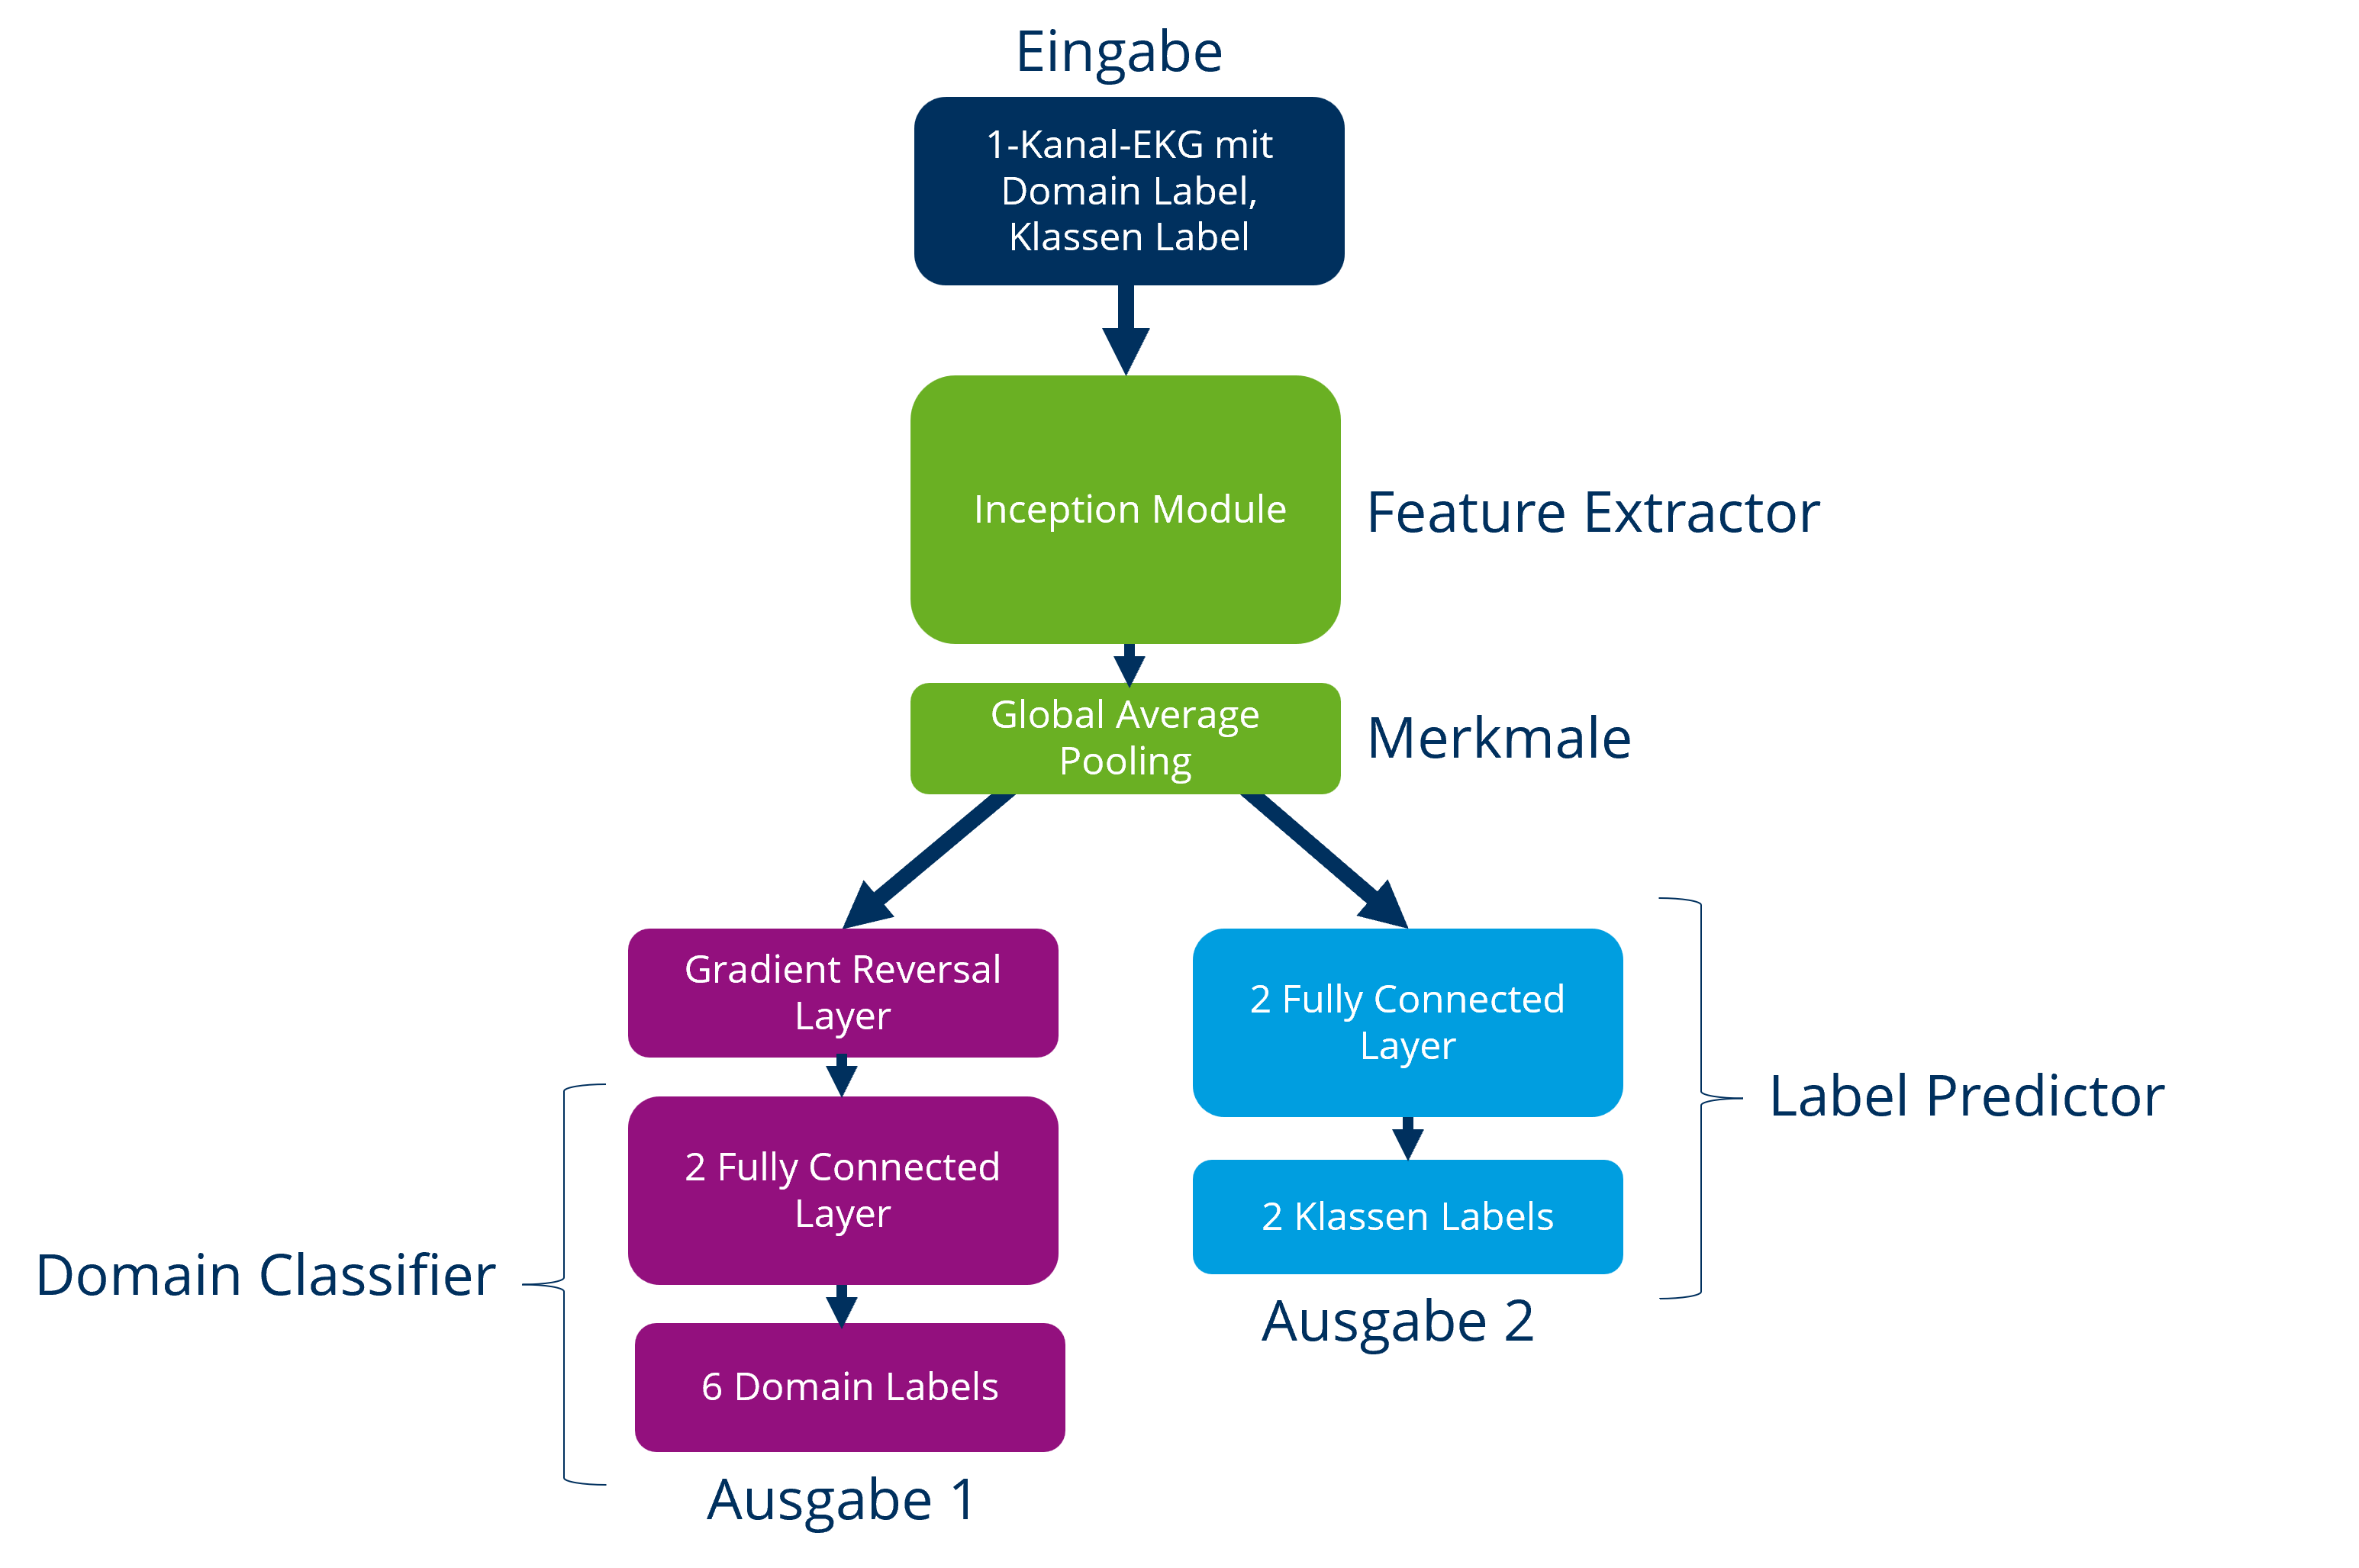
\includegraphics[width=1\textwidth]{./Bilder/DANN_architektur.png}
\caption[DANN Architektur]{Architektur des \gls{DANN}s. Als Eingabe dienen 1-Kanal-\gls{EKG}s. Als Feature Extractor dient InceptionTime. Für den Domain Classifier wird an den \gls{GAP}-Layer der \gls{GRL} angeschlossen, worauf zwei \gls{FC}-Layer folgen. Die Ausgabeschicht des Domain Classifiers besitzt 6 Neuronen für die 6 Domänen. Der Label Predictor besitzt 2 \gls{FC}-Layer angeschlossen an den \gls{GAP}-Layer und 2 Neuronen als Ausgabeschicht für die zwei Zielklassen \gls{VHF} und nicht-\gls{VHF}.} 
\label{fig:DANN}
\end{figure} 

\subsection*{DANN mit Direktausgabe der Merkmale}

Zur Untersuchung des Einflusses der Feature-Transformation, die in den \gls{FC}-Layern stattfindet, auf die Generalisierungsfähigkeit des Modells wird ein \gls{DANN} ohne \gls{FC}-Layer zwischen \gls{GAP}-Layer und Ausgabeschicht im Label Predictor trainiert. Dadurch werden die Merkmale aus dem Feature Extractor ohne Zwischenrepräsentationen direkt ausgegeben. Diese Version des \gls{DANN}s wird im weiteren Verlauf der Arbeit als DANNdirect bezeichnet und ist in \hyperref[fig:DANNdirect]{Abb.~5.2} dargestellt.

\begin{figure}[!ht]%
\centering
	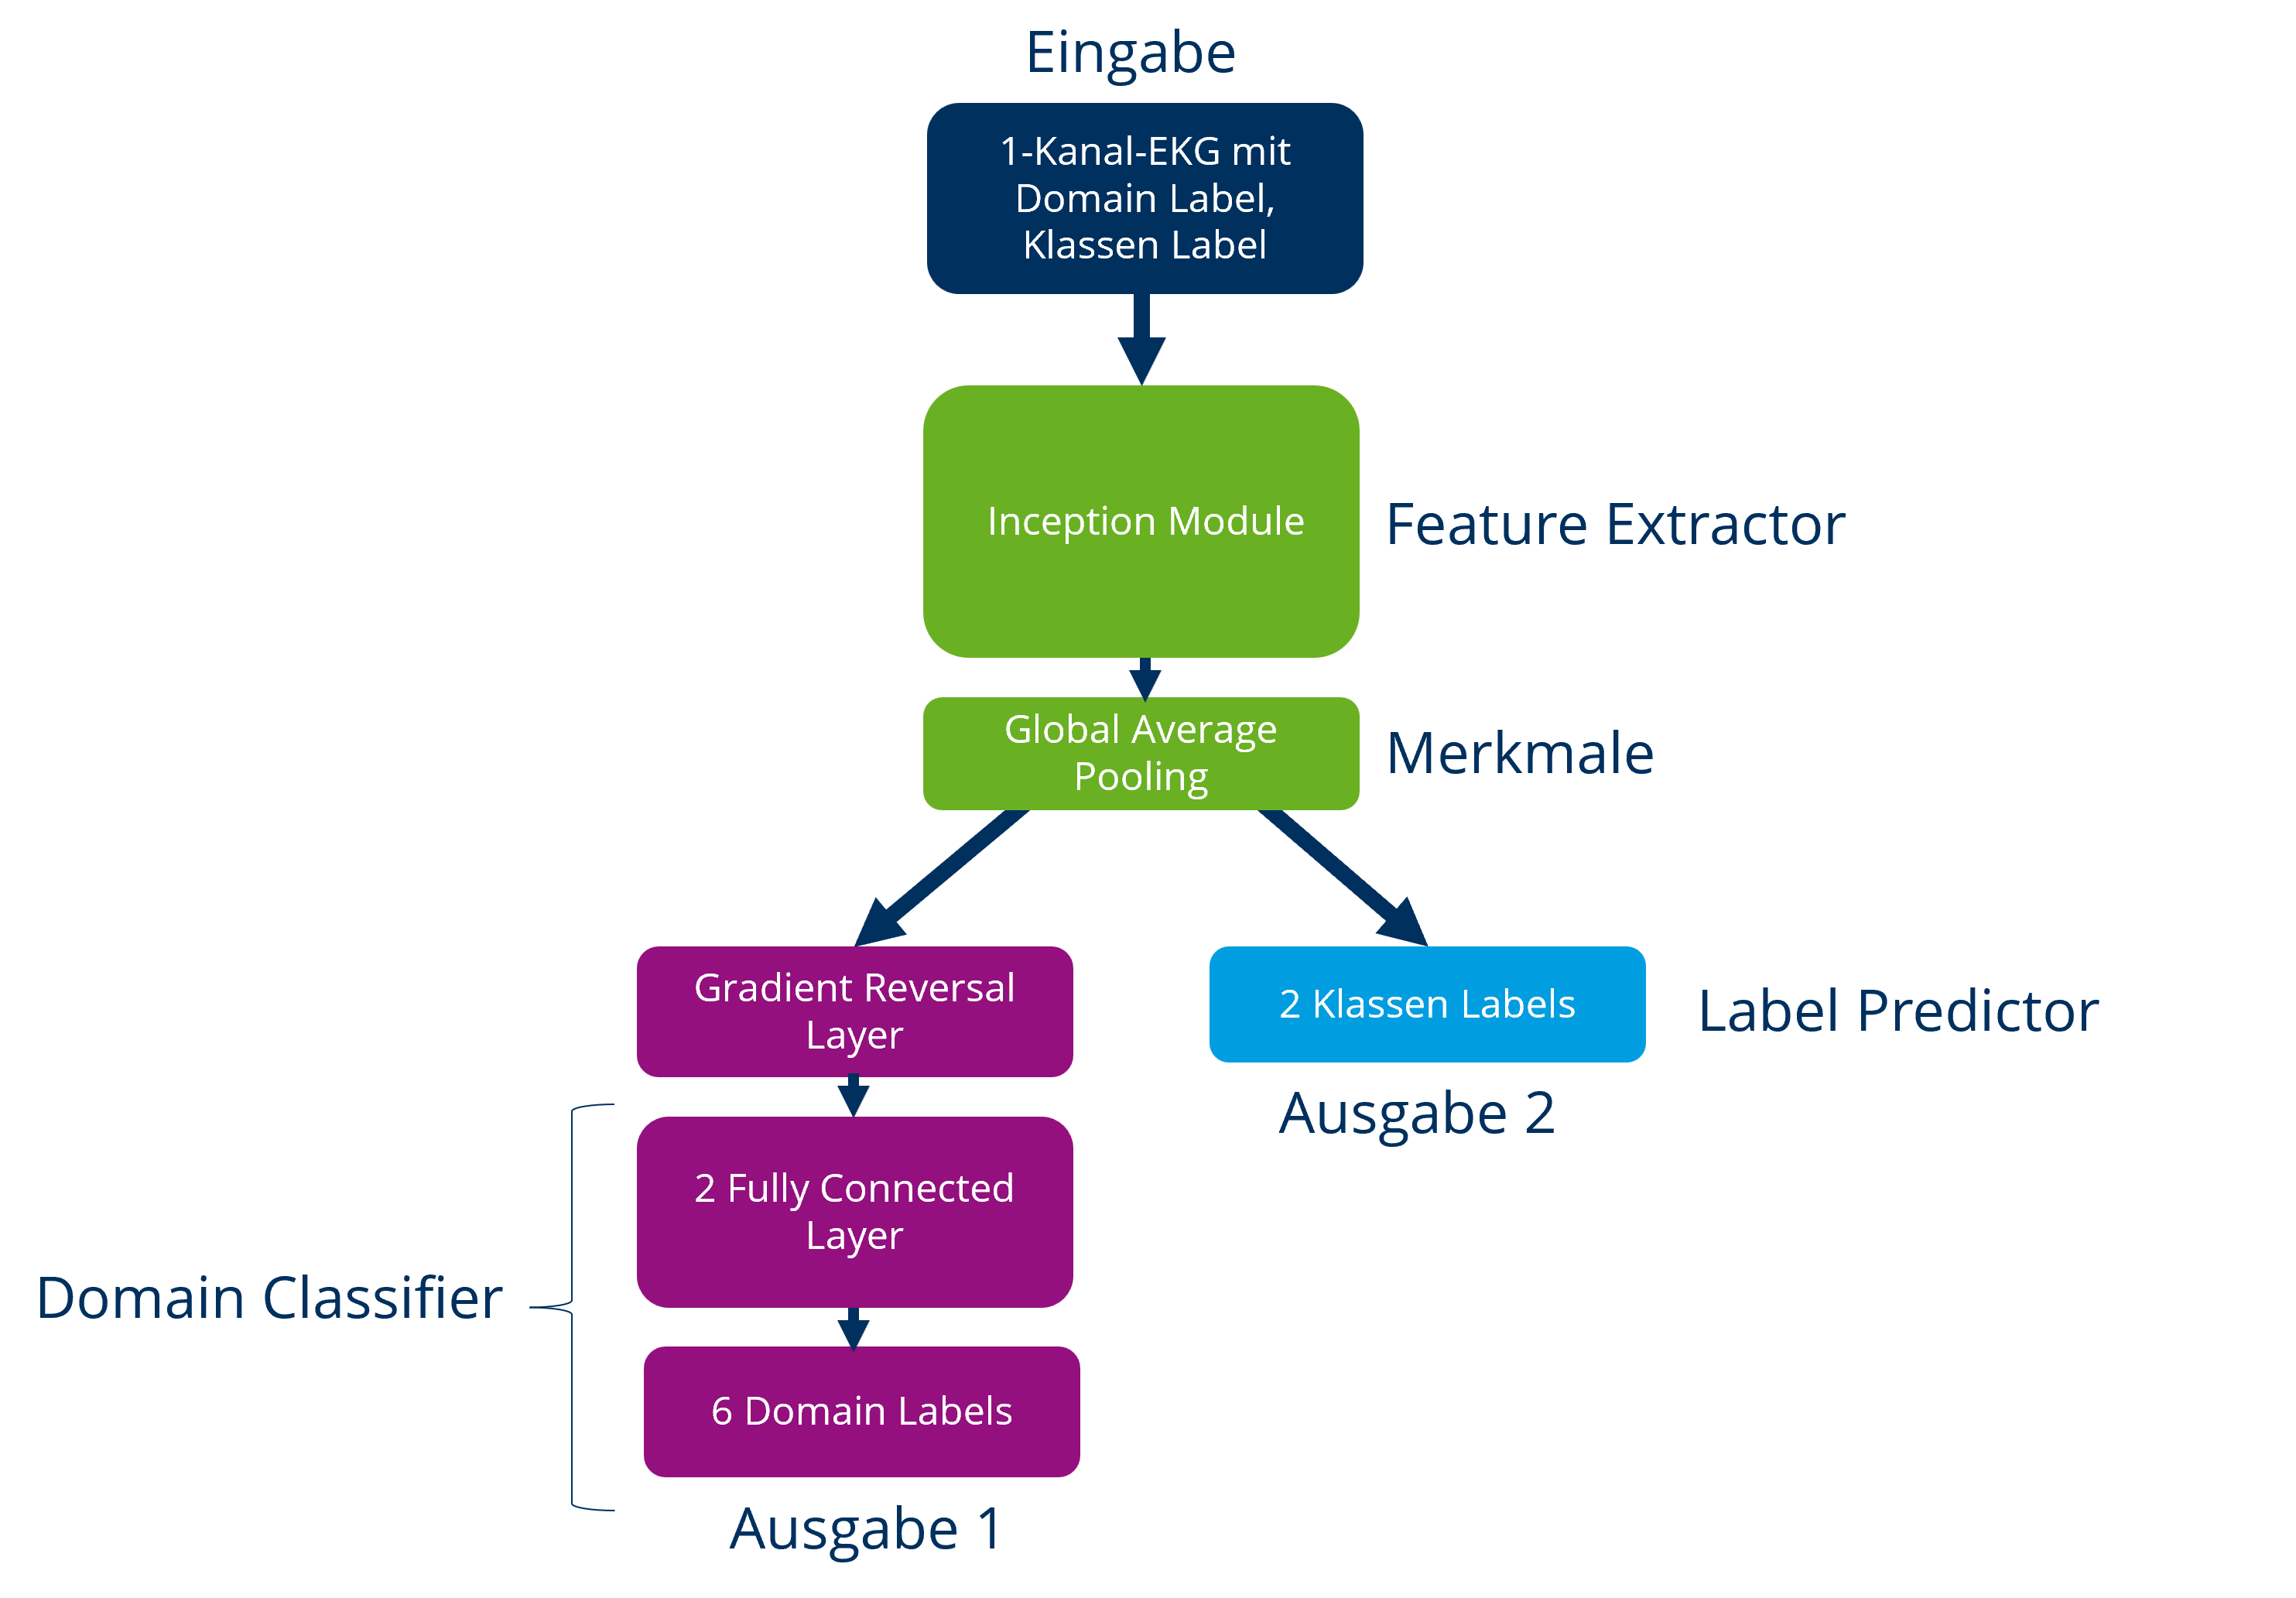
\includegraphics[width=1\textwidth]{./Bilder/DANNdirect_architektur.png}
\caption[DANNdirect Architektur]{Architektur des \gls{DANN}direct Modells. Als Eingabe dienen 1-Kanal-\gls{EKG}s. Als Feature Extractor dient InceptionTime. Für den Domain Classifier wird an den \gls{GAP}-Schicht den \gls{GRL} angeschlossen, worauf zwei \gls{FC}-Layer folgen. Die Ausgabeschicht des Domain Classifiers besitzt 6 Neuronen für die 6 Domänen. Der Label Predictor besitzt 2 Neuronen als Ausgabeschicht für die zwei Zielklassen \gls{VHF} und nicht-\gls{VHF}. } 
\label{fig:DANNdirect}
\end{figure} 


\subsection*{Vergleichsmodell InceptionTime}

Als Vergleichsmodell wurde ein wie in \hyperref[sec:InceptionTime]{Kapitel 4.1} beschriebenes klassisches InceptionTime-Ensemble  gewählt. Wie auch beim Feature Extractor des \gls{DANN}s sind in den Inception Modulen jeweils 3 Filtersets mit 32 Filtern mit den Filtergrößen $l \in \{10, 20, 40\}$ enthalten. Auch beim Vergleichsmodell wurde die Anzahl der Inception Module per Grid Search ermittelt.

Für alle drei genannten Architekturen wird das Ensemble aus 5 Modellen erstellt, welche gleich gewichtet eine Mehrheitsentscheidung für die \gls{VHF}-Klassifkation treffen, wie es von Fawaz~et~al.~\cite{fawaz_inceptiontime_2020} für InceptionTime empfohlen wird. Zusätzlich wird ein Ensembleergebnis gewichtet bestimmt, indem die jeweiligen Sicherheiten gemittelt werden und mittels \texttt{argmax} die Klasse bestimmt wird, sodass Modelle, die sich sicherer in ihrer Entscheidung sind, mehr zum Endergebnis beitragen. Die 5 Modelle stammen aus der 5-fold Cross Validation (siehe \hyperref[sec:trainingsprozess]{Abschnitt 5.4}) und sind somit auf teilweise unterschiedlichen Daten trainiert. 


\section{Trainings- und Optimierungsprozess}\label{sec:trainingsprozess}


Das Training der Modelle fand auf dem \gls{HPC} der Technischen Universität Dresden statt. Genutzt wurde das GPU-Cluster \texttt{Alpha Centauri}, welches AMD EPYC CPUs und NVIDIA A100-SXM4 GPUs besitzt. Die lokale Entwicklung und die Evaluation der Modelle fand auf einer NVIDIA GeForce RTX 3070 Laptop GPU statt. Programmiert wurde in \texttt{Python 3.10}, genutzte Frameworks sind \texttt{aeon 0.11.1}, \texttt{tensorflow-gpu 2.9.0} und \texttt{keras 2.9.0}. \texttt{Aeon} wird zum Import der \texttt{IndividualInceptionTimeClassifier} genutzt.

Für das Training des \gls{DANN}s und DANNdirects wurde der Adam Optimizer genutzt. Der beim Training beobachtete Loss ist der ungewichtete kombinierte Loss aus dem Label Predictor Loss und dem Domain Classifier Loss. Das Training wurde per Early Stopping beendet, wenn für 20 Epochen keine weitere Verringerung im Loss des Label Predictors auftrat. Für das Training wurde ein absoluter Grenzwert von 500 Epochen gewählt.
Die Hyperparameteroptimierung wurde per Grid Search durchgeführt. Optimiert wurden die Hyperparameter \texttt{batch size = [32, 64, 128]}, \texttt{learning rate = [0.01, 0.001, 0.0001]} und Anzahl der Inception-Module, bezeichnet als \texttt{depth = [3, 6, 9]}. Die Konstante des \gls{GRL}s wird auf 1 gesetzt, sodass der Gradient des Domain Classifiers während der Backpropagation vollständig invertiert wird.

Obwohl nach Ganin et al. \cite{ganin_domain-adversarial_2016} für Domain Adversarial Learning keine Domain Labels nötig sind, wird in diesem Ansatz vollständig supervised Learning genutzt, da Domain Labels in Form der jeweiligen Ableitungen I, II, III, aVR, aVL und aVF der \gls{EKG}-Signale vorhanden sind. Die Zielklassen des Label Predictors sind \gls{VHF} und nicht-\gls{VHF}. Zur Validierung während des Trainings wird 5-fold Cross Validation mit balancierten Klassen (siehe \hyperref[tab:folds]{Tab. 5.5}) sowohl in den Zielklassen als auch in den Domain-Klassen genutzt. Die Modelle, die während der 5-fold Cross Validation trainiert wurden, werden für das Ensemble genutzt.

Für das Training der InceptionTime-Modelle werden dieselben Werte in der Hyperparameteroptimierung angepasst. Das Training wird ebenfalls per Early Stopping beendet, sobald der Loss der InceptionTime-Ausgabe nach 20 Epochen nicht weiter gesunken ist. Für das Training wurde ein absoluter Grenzwert von 500 Epochen gewählt. Zur Validierung wird ebenfalls 5-fold Cross Validation genutzt. Die Modelle, die während der Cross Validation trainiert wurden, werden für das Ensemble genutzt. Trainingsklassen sind \gls{VHF} und nicht-\gls{VHF}.


\begin{table}[h!]
\centering
\caption[Klassenverteilung Cross Validation]{Verteilung der Trainings- und Validierungslabels für Vorhofflimmern (VHF) und Domains in der Cross Validation.}
\label{tab:folds}
%\scalebox{0.8}{
\begin{tabular}{llcccccc}
\toprule
\textbf{Fold} & \textbf{Datensatz} &  &  & \textbf{Klasse} &  &  &  \\
\midrule
\textbf{Fold 1} & & nicht-VHF & VHF & & & &\\
\cmidrule{2-8}
	   & Training VHF       & 21367 & 21199 & - & - & - & - \\
       & Validation VHF     & 5321 & 5321 & - & - & - & - \\
\cmidrule{3-8}
       & & I & II & III & aVR & aVL & aVF \\
\cmidrule{3-8}
       & Training Domain    & 7077 & 7127 & 7141 & 7103 & 7057 & 7061 \\
       & Validation Domain  & 1791 & 1741 & 1727 & 1765 & 1811 & 1807 \\
\midrule

\textbf{Fold 2} & & nicht-VHF & VHF & & & &\\
\cmidrule{2-8}
	   & Training VHF       & 21394 & 21172 & - & - & - & - \\
       & Validation VHF     & 5294 & 5348 & - & - & - & - \\
\cmidrule{3-8}
       & & I & II & III & aVR & aVL & aVF \\
\cmidrule{3-8}
       & Training Domain    & 7090 & 7104 & 7033 & 7063 & 7148 & 7128 \\
       & Validation Domain  & 1778 & 1764 & 1835 & 1805 & 1720 & 1740 \\
\midrule


\textbf{Fold 3} & & nicht-VHF & VHF & & & &\\
\cmidrule{2-8}
	   & Training VHF       & 21316 & 21250 & - & - & - & - \\
       & Validation VHF     & 5372 & 5270 & - & - & - & - \\
\cmidrule{3-8}
       & & I & II & III & aVR & aVL & aVF \\
\cmidrule{3-8}
       & Training Domain    & 7086 & 7073 & 7079 & 7153 & 7054 & 7121 \\
       & Validation Domain  & 1782 & 1795 & 1789 & 1715 & 1814 & 1747 \\
\midrule


\textbf{Fold 4} & & nicht-VHF & VHF & & & &\\
\cmidrule{2-8}
	   & Training VHF       & 21294 & 21273 & - & - & - & - \\
       & Validation VHF     & 5394 & 5247 & - & - & - & - \\
\cmidrule{3-8}
       & & I & II & III & aVR & aVL & aVF \\
\cmidrule{3-8}
       & Training Domain    & 7090 & 7117 & 7134 & 7144 & 7042 & 7040 \\
       & Validation Domain  & 1778 & 1751 & 1734 & 1724 & 1826 & 1828 \\
\midrule

\textbf{Fold 5} & & nicht-VHF & VHF & & & &\\
\cmidrule{2-8}
	   & Training VHF       & 21381 & 21186 & - & - & - & - \\
       & Validation VHF     & 5307 & 5334 & - & - & - & - \\
\cmidrule{3-8}
       & & I & II & III & aVR & aVL & aVF \\
\cmidrule{3-8}
       & Training Domain    & 7129 & 7051 & 7085 & 7009 & 7171 & 7122 \\
       & Validation Domain  & 1739 & 1817 & 1783 & 1859 & 1697 & 1746 \\

\bottomrule
\end{tabular}
%}
\end{table}

